\documentclass[tikz,border=10pt]{standalone}
\usepackage{tkz-graph}
\usepackage{amsmath,amssymb}
\usepackage{xcolor}
\usetikzlibrary{calc}
\usetikzlibrary{positioning}
\usetikzlibrary{shadings}

% Chapter 7: Filling,Climbing, and Shading
\begin{document}

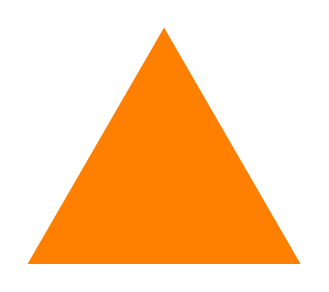
\begin{tikzpicture}
	\path[fill=orange] (90:2) -- (210:2) -- (330:2) -- cycle;
\end{tikzpicture}



\begin{tikzpicture}
	\path[fill=orange]  (150:1) -- (210:2) -- (330:2) -- (30:1) -- (0, -.5) -- cycle;
\end{tikzpicture}

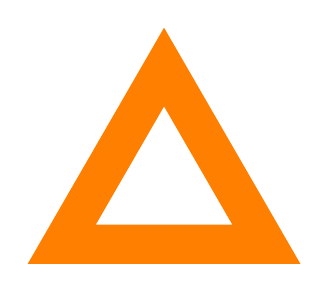
\begin{tikzpicture}
	\fill[orange, even odd rule]
	(90:2) -- (210:2) -- (330:2) -- cycle
	(90:1) -- (210:1) -- (330:1) -- cycle;
\end{tikzpicture}


\begin{tikzpicture}
	\fill[blue!50, even odd rule](90:1) -- (234:1) -- (18:1) -- (162:1) -- (306:1) -- cycle;
\end{tikzpicture}


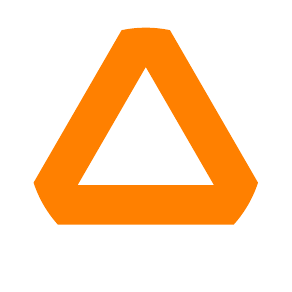
\begin{tikzpicture}
	\clip[] (0,0) circle (1.5);
	\fill[orange]
	(90:2) -- (210:2) -- (330:2) -- cycle
	(90:1) -- (330:1) -- (210:1) -- cycle;
\end{tikzpicture}

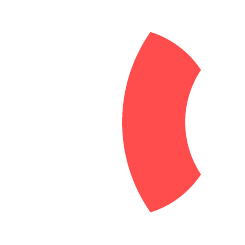
\begin{tikzpicture}[even odd rule]
	% \clip (-3, 0) rectangle (3,2);
	\clip (-1,0) circle (1.2);
	\fill[red!70] (1,0) circle (1.2) (1,0) circle (2);
\end{tikzpicture}

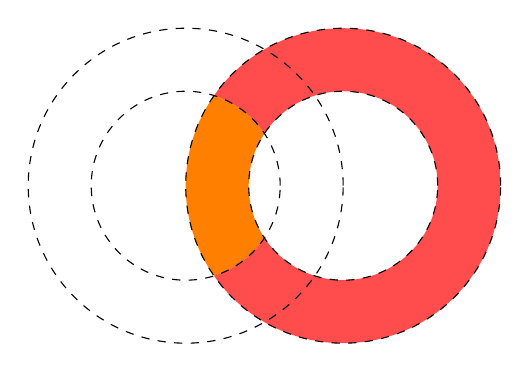
\begin{tikzpicture}[even odd rule]
	\begin{scope}
		\clip (-1,0) circle (1.2);
		\fill[orange] (1,0) circle (1.2) (1,0) circle (2);
	\end{scope}

	\begin{scope}
		\clip[overlay] (-1,0) circle (1.2) (-2,-2) rectangle (3,2);
		\fill[red!70] (1,0) circle (1.2) (1,0) circle (2);
	\end{scope}

	\draw[dashed] (-1,0) circle (1.2) (-1,0) circle (2);
	\draw[dashed] (1,0) circle (1.2) (1,0) circle (2);
\end{tikzpicture}

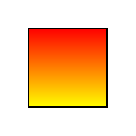
\begin{tikzpicture}
	\shadedraw [top color=red, bottom color=yellow] (0,0) rectangle (1,1);
\end{tikzpicture}

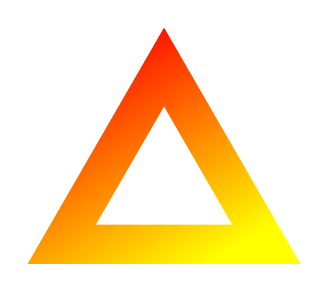
\begin{tikzpicture}
	\shade[top color=red, bottom color=yellow, shading angle=30]
	(90:2) -- (210:2) -- (330:2) -- cycle
	(90:1) -- (330:1) -- (210:1) -- cycle;
\end{tikzpicture}

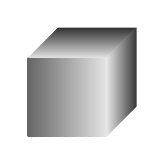
\begin{tikzpicture}
	\shade[left color=black!60, right color=black!10]
	(0,0,0) -- (1,0,0) -- (1,1,0) -- (0,1,0);
	\shade[left color=black!10, right color=black!80]
	(1,0,0) -- (1,0,-1) -- (1,1,-1) -- (1,1,0);
	\shade[bottom color=black!10, top color=black!80]
	(0,1,0) -- (0,1,-1) -- (1,1,-1) -- (1,1,0);
\end{tikzpicture}


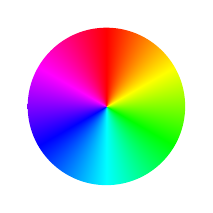
\begin{tikzpicture}
	\shade[shading=color wheel] (0,0) circle (1);
\end{tikzpicture}


\end{document}

